\chapter{Diseño e implementación} % Main chapter title

\label{Chapter3} % Change X to a consecutive number; for referencing this chapter elsewhere, use \ref{ChapterX}

\definecolor{mygreen}{rgb}{0,0.6,0}
\definecolor{mygray}{rgb}{0.5,0.5,0.5}
\definecolor{mymauve}{rgb}{0.58,0,0.82}

%%%%%%%%%%%%%%%%%%%%%%%%%%%%%%%%%%%%%%%%%%%%%%%%%%%%%%%%%%%%%%%%%%%%%%%%%%%%%
% parámetros para configurar el formato del código en los entornos lstlisting
%%%%%%%%%%%%%%%%%%%%%%%%%%%%%%%%%%%%%%%%%%%%%%%%%%%%%%%%%%%%%%%%%%%%%%%%%%%%%
\lstset{ %
  backgroundcolor=\color{white},   % choose the background color; you must add \usepackage{color} or \usepackage{xcolor}
  basicstyle=\footnotesize,        % the size of the fonts that are used for the code
  breakatwhitespace=false,         % sets if automatic breaks should only happen at whitespace
  breaklines=true,                 % sets automatic line breaking
  captionpos=b,                    % sets the caption-position to bottom
  commentstyle=\color{mygreen},    % comment style
  deletekeywords={...},            % if you want to delete keywords from the given language
  %escapeinside={\%*}{*)},          % if you want to add LaTeX within your code
  %extendedchars=true,              % lets you use non-ASCII characters; for 8-bits encodings only, does not work with UTF-8
  %frame=single,	                % adds a frame around the code
  keepspaces=true,                 % keeps spaces in text, useful for keeping indentation of code (possibly needs columns=flexible)
  keywordstyle=\color{blue},       % keyword style
  language=[ANSI]C,                % the language of the code
  %otherkeywords={*,...},           % if you want to add more keywords to the set
  numbers=left,                    % where to put the line-numbers; possible values are (none, left, right)
  numbersep=5pt,                   % how far the line-numbers are from the code
  numberstyle=\tiny\color{mygray}, % the style that is used for the line-numbers
  rulecolor=\color{black},         % if not set, the frame-color may be changed on line-breaks within not-black text (e.g. comments (green here))
  showspaces=false,                % show spaces everywhere adding particular underscores; it overrides 'showstringspaces'
  showstringspaces=false,          % underline spaces within strings only
  showtabs=false,                  % show tabs within strings adding particular underscores
  stepnumber=1,                    % the step between two line-numbers. If it's 1, each line will be numbered
  stringstyle=\color{mymauve},     % string literal style
  tabsize=2,	                   % sets default tabsize to 2 spaces
  title=\lstname,                  % show the filename of files included with \lstinputlisting; also try caption instead of title
  morecomment=[s]{/*}{*/}
}


%----------------------------------------------------------------------------------------
%	SECTION 1
%----------------------------------------------------------------------------------------
\section{Análisis del software}

\subsection{Arquitectura del sistema}
La solución esta integrada por 6 componentes principales. La interfaz visual, diseñada en Unity3D, a través de la cual el usuario interactúa con la aplicación. El backend de esta interfaz, desarrollado en .NET utilizando CSharp como lenguaje de programación. La APIrest, a través de la cual la aplicación embebida en el Hololens2 se comunica con el servidor web. La base de datos, que es actualizada a través de la APIrest. El servicio OPC, desde el cual se enviarán los datos pertinentes al sistema de control, a través del \textit{standard} industrial OPC. Y finalmente el sistema de control, representado por un controlador simulado. En la Figura \ref{fig:Diag_bloques} se puede observar el diagrama en bloques:

\begin{figure}[htpb]
	\centering
	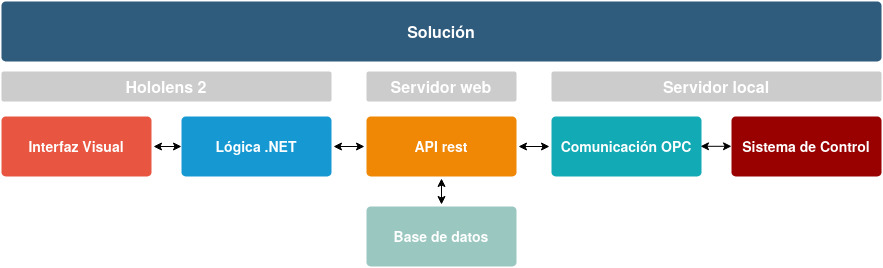
\includegraphics[scale=.5]{./Figures/Diag_bloques.jpg}
	\caption{diagrama en bloques\protect\footnotemark.}
	\label{fig:Diag_bloques}
\end{figure}

Imagen de elementos en la DB
Imagen de lo devuelto por la api
Imagen SFC control

\subsection{Interfaz de realidad aumentada}
\subsubsection{Aplicación}

La aplicación se encarga de ayudar a los operadores durante la fabricación por lotes de un producto determinado. Durante los procedimientos \textit{batch} se utilizan el mismo conjunto de maquinas para la fabricación de distintos productos. Por lo tanto, las tareas de los operadores varían en las distintas partes del proceso dependiendo del producto que se este fabricando. Una etapa clave en la fabricación del producto, es el agregado de aditivos en la mezcla. La aplicación desarrollada se encarga de evitar que el operador falle a la hora de seleccionar y dosificar el aditivo requerido. La aplicación comienza con la siguiente imagen:
producir

En este punto se aguarda la lectura del codigo QR correspondiente a la receta a producir. Las recetas son el conjunto de parámetros que involucran un lote de producción. En ellas podemos encontrar el listado de aditivos, la cantidades requeridas, los códigos de los distintos productos, tiempos de mezclado y demás parámetros necesarios para la producción. Si el operador lee un código de receta para el cual, el sistema de control no fue configurado a producir en ese momento, se indicara un error como muestra la siguiente figura:

Para poder avanzar, es necesario que se lea el código de la receta correcta. Como podemos ver a continuación: 

En este punto el operador acepta la receta y la interfaz mostrara la siguiente imagen:


En el margen derecho podemos ver 3 círculos azules, los cuales representan 3 tareas del operador a lo largo de la receta de producción. En la parte superior del listado de tareas podemos leer el producto que se fabricara en esta receta. En el lado izquierdo superior podemos ver una leyenda que ira actualizándose para guiar al operador. En la parte inferior encontramos 4 botones con las siguientes funcionalidades:

\begin{itemize}
\item Ocultar: permite simplificar la vista holográfica, reduciendo la información proyectada en el hololens.
\item Mostrar: restablece la información holográfica oculta.
\item Datos: restablece la información correspondiente a la lecrestablece la información holográfica oculta.tura de codigos QR. 
\item Siguiente: se utiliza para avanzar a la siguiente etapa drestablece la información holográfica oculta.e producción. 
\end{itemize}

Ademas en el centro izquierdo de la imagen, podemos ver datos que hacen referencia a los distintos aditivos que se usaran en la receta. Se muestran los siguientes datos:

\begin{itemize}
\item QR: código QR leído por el hololens.
\item Código: código del producto leído .
\item Producto: nombre del producto leído. 
\item Cantidad: cantidad necesaria del producto en la receta.
\end{itemize}

Según lo indicado en pantalla el operador deberá pulsar ``Siguiente'' para iniciar el procedimiento. En ese momento la instrucción se modificara, solicitándole que vierta en el tanque de producción TK212, el producto A. Como podemos ver en la siguiente imagen:


El operador deberá localizar las bolsas de este producto y leerá con el Hololens el código QR de la misma. En ese momento el conjunto de datos de actualizara como vemos en la siguiente figura:


El operador pulsara ``Aceptar'' y luego deberá  ingresar las cantidades indicadas en el tanque de producción. Luego pulsara ``Siguiente'' y se actualizara la información con una nueva instrucción como vemos a continuación:

Si el operador hubiese cometido un error al tomar la bolsa de un producto no requerido, la siguiente imagen hubiese alertado al operador, y no hubiese podido avanzar la receta de ninguna manera:


El procedimiento se repetirá para el total de las tareas de la receta. Hasta la ultima operación, luego se mostrara la siguiente imagen indicándole al operador que puede cerrar la aplicación:


Los comandos al sistema de control son enviados luego de que el correcto producto fue leído y el operador avanza al siguiente paso de la receta, garantizando que se cumplió la tarea asignada. Si el producto erróneo es leído, el operador no tiene habilitado el paso siguiente, por lo tanto queda retenido en esa etapa. Ademas, las recetas validas son solo aquellas en las que el sistema de control aguarda operaciones manuales, de esta manera nos aseguramos que no puedan mezclarse otras recetas con la receta activa.

\subsubsection{API y base de datos}
La API (\textit{Application Programming Interface}) fue desarrollada en .NET y se implementaron las siguientes operaciones:

\begin{itemize}
\item GET: 
\item POST: 
\item PATCH:
\item DELETE:
\end{itemize}

Se creo una clase ``Receta'' la cual contiene los siguientes parámetros:

\begin{itemize}
\item 1: 
\item 2:
\item 3:
\end{itemize}

Esta clase también se implemento en la lógica del Hololens. De esta manera, se utilizan los metodos GET y PATCH durante los pasos de la interfaz para adquirir o enviar datos a la API. Cuando desde la interfaz leemos un código QR, internamente estamos enviando una petición GET al servidor web, para traer los datos de la receta y almacenarlos en una instancia de la clase Receta. Si la receta es correcta, utilizaremos el mismo ID de receta, para enviar las actualizaciones de estado cuando el operador avance una etapa. Esta actualización se hace con el verbo PATCH. Este se implemento para modificar solo los parámetros del input de usuario en la receta y no alterar el resto. 

La API se hosteo en Azure, la plataforma \textit{cloud} de Microsoft. Se utilizo el servicio Azure Web Apps, que es una plataforma que permite publicar aplicaciones web que se ejecutan en múltiples \textit{frameworks} y escritas en diferentes lenguajes de programación. Esto permitió aumentar la velocidad de desarrollo de la aplicación dado que la sincronización y el \textit{deployment} son prácticamente instantáneos. Ademas, ofrece múltiples posibilidades de integración con otros servicios a futuro.

El motor de la base de datos utilizado es MongoDB. Es una base de datos NoSQL basada en documentos. Se opto por esta tecnología dado que los parámetros de las recetas podían ser encapsulados en un JSON . Se utilizo la plataforma SaaS de MongoDB, Atlas, para poder brindar flexibilidad y escalabilidad a la solución con una base de datos cloud. Para acceder a la misma se debe utilizar una \textit{key} que solo posee la APIrest. A continuación se muestra la colección de datos creada para la aplicación:

Imagen de mongodb

\subsection{Sistema de control}
\subsubsection{Nodo 800xA}
Para el sistema de control se utilizo la herramienta de ABB denominada \textit{SoftController}. Esta nos permite simular la presencia de un controlador físico conectado a la red, con la IP del localhost. Para la lógica de control se uso el CBM (\textit{Compact Control Builder}) , que nos permite crear lógicas del mismo tipo que las usadas en los sistemas DCS 800xA de ABB. De hecho las mismas podrían exportarse al sistema 800xA sin problemas. A continuación podemos ver una imagen del \textit{SoftController} simulando un controlador:

En el CBM podemos ver los bloques de las distintas recetas en la aplicación de control, como se muestra en esta figura:


A medida que nuevas recetas sean necesarias, estos bloques funcionan como objetos de una clase que pueden instanciarse para cada tipo de receta. Simultáneamente estas recetas se cargan en la base de datos para establecer la comunicación entre el sistema de control y la interfaz del Hololens. Dentro de la receta podemos ver una lógica secuencial del procedimiento, que ira avanzando a medida que el operador complete los pasos en la interfaz holográfica. Podemos ver una imagen del avance de la secuencia en el tiempo:

Por ultimo tenemos el OPC server. Esta aplicación crea un OPC server con acceso a las variables del sistema de control. Para conectarnos debemos apuntar a la IP del controlador simulado como se muestra a continuación:

Este nodo se implemento en una maquina virtual usando VirtualBox, posee un sistema operativo Windows 10 con 4 gb de memoria RAM y 60 Gb de disco. La ventaja radica en la portabilidad del nodo, dado que podría integrarse a un servidor ESXI en cualquier entorno industrial. 

\subsubsection{Servicio de actualización}

El servicio se instalo en el mismo nodo virtualizado 800xA visto anteriormente. Se encarga de actualizar la base de datos según los cambios en el sistema de control. Y viceversa, también es capaz de actualizar las variables de control de acuerdo a la base de datos. Se desarrollo en .NET y se ejecuta  como un servicio mas de Windows. El servicio incluye el \textit{framework} OPC mencionado en el Capitulo 2, lo que le permite leer y escribir variables OPC. 

Una vez en ejecución se encarga de realizar consultas GET a la APIrest de cada una de las recetas en ejecución. De esta manera es capaz de detectar que los insumos ya fueron vertidos en el tanque y avanzar así a la siguiente etapa. Ademas, se encarga de setear la variable ``waitinput'', la misma es clave en el funcionamiento de la aplicación dado que indica que la receta se encuentra en ejecución y aguarda ordenes del operador. De esta manera se valida que el operador solo pueda iniciar la aplicación con la receta en ejecución por mas que intente leer otros códigos de receta inválidos. 

A continuación podemos ver el código de la implementación de los métodos OPC:

\begin{lstlisting}[label=cod:vControl,caption=Pseudocódigo del lazo principal de control.]  % Start your code-block

#define MAX_SENSOR_NUMBER 3
#define MAX_ALARM_NUMBER  6
#define MAX_ACTUATOR_NUMBER 6

uint32_t sensorValue[MAX_SENSOR_NUMBER];		
FunctionalState alarmControl[MAX_ALARM_NUMBER];	//ENABLE or DISABLE
state_t alarmState[MAX_ALARM_NUMBER];						//ON or OFF
state_t actuatorState[MAX_ACTUATOR_NUMBER];			//ON or OFF

void vControl() {

	initGlobalVariables();
	
	period = 500 ms;
		
	while(1) {

		ticks = xTaskGetTickCount();
		
		updateSensors();
		
		updateAlarms();
		
		controlActuators();
		
		vTaskDelayUntil(&ticks, period);
	}
}

\end{lstlisting}



